%moteurs
\subsection{Le dimensionnement en régime permanent}
%~~~~~~~~~~~~~~~~~~~~~~~~~~~~~~~~~~~~~~~~~~~~~~~~~~~~~~~~~~~~
La force motrice doit être égale à la force résistante, par le principe de la somme des forces:

$$Fm - Fr = m \times \overrightarrow{a}$$

En régime permanent l’accélération est nulle :

$$Fm = Fr = \mu \times m \times g$$

$\mu = 0.15$, coefficient de frottement de la roue sur la table ;

$m = 10 kg$, le poids max du robot;

$g = 9.81 \frac{m}{s^{2}}$, accélération de pesanteur.

\paragraph{}
On peut donc trouver directement le couple qu’il faut à la roue pour faire avancer le robot :

$$Croue = Fr \times r = 14.715N \times 0.04m = 588,6 mNm$$

On utilise un réducteur pour réduire la vitesse de rotation du moteur,  la puissance étant conservée $P = C \times W$ donc le couple récupérer à la sortie est multiplié  par le rapport de réduction :

$$Cmoteur= \frac {Croue}{rapport de reduction} = \frac {588.6 mNm} {20} = 29.43 mNm$$

La vitesse max du robot est de $5 \frac{km}{h}$ ce qui correspond a $1.38 \frac{m}{s}$ :

$$\omega roue = \frac{v}{r}= \frac{1.388 \frac{m}{s}}{0.04m}= 34.7 \frac{rad}{s} $$

$$Nroue = \frac {\omega} {2 \pi } \times 60 = 331.57 \frac {tr}{min}$$

$$P = Cm \times \omega m = 694 \frac {rad}{s}  \times 0.02943 N = 20.42 W$$
   
\subsection{Le dimensionnement à l'accélération}
%~~~~~~~~~~~~~~~~~~~~~~~~~~~~~~~~~~~~~~~~~~~~~~~~~~~~~~~~~~~~
$$Fm - Fr = m \times \overrightarrow{a}$$

On suppose que l'on atteindra la vitesse du régime, c’est-à-dire 1.38 m/s en 1 s :

$$Fm - Fr = m \times \overrightarrow{a} = 10 kg \times 1.38 \frac{m}{s^{2}} = 13.8 N$$

$$Fm =Fr + 13.8 N = 13.8 + 17.715 = 28.5 N$$
  
$Croue = Fr \times r = 28.5 N  \times 0.04m = 1.14 Nm$ , $r = 0.04m$ (rayon de la roue)

$$Cmoteur = \frac {Croue}{20} = 57 mNm$$

La vitesse angulaire du moteur reste la même dans les deux régimes :

$$P = Cm \times Wm = 0.057 mNm \times 694 \frac {rad}{s} = 39.7 W$$

\subsection{Conclusions}
%~~~~~~~~~~~~~~~~~~~~~~~~~~~~~~~~~~~~~~~~~~~~~~~~~~~~~~~~~~~~
On a choisi nos moteurs par rapport au régime le plus contraignant c’est à dire en tenant compte de l’accélération pour que nous ne soyons limité d'aucune manière.
  
\noindent Nous avons donc cherché dans le catalogue pour trouver le moteur qui convient le mieux à nos critères et finalement nous avons pris deux moteurs Maxon \textit{RE-max 29} à commutation graphite de {22 Watts} modèle : 226806. La fiche technique est montrée à la page suivante.

\noindent Nous avons choisi aussi un réducteur $1:21$ modèle n : 166160, et le codeur n 225805 dont les figures~\ref{img:moteur},~\ref{img:gearhead} et~\ref{img:encoder} sont les fiches techniques.

\noindent Notre choix a été appuyé par la \textit{tension d’alimentation du moteur (24 V)}, qui est facilement disponible ainsi que le {couple nominal du moteur}.

\begin{figure}[!hp]
	\centering
	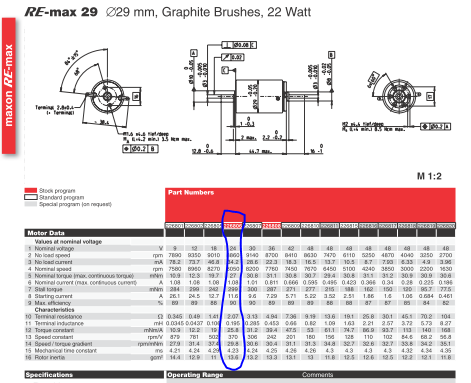
\includegraphics[width=15cm]{Moteur.PNG}
	\caption{Choix du moteur}
	\label{img:moteur}
\end{figure}

\begin{figure}[!hp]
	\centering
	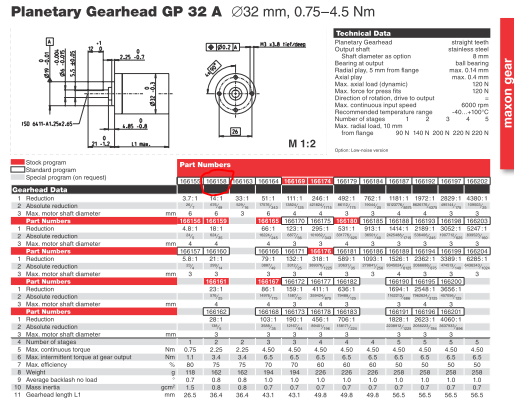
\includegraphics[width=15cm]{Gearhead.PNG}
	\caption{Choix du gearhead}
	\label{img:gearhead}
\end{figure}

\begin{figure}[!hp]
	\centering
	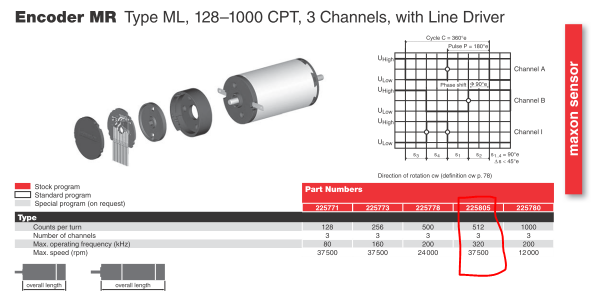
\includegraphics[width=15cm]{Encoder.PNG}
	\caption{Choix de l'encodeur}
	\label{img:encoder}
\end{figure}

%@@@@@@@@@@@@@@@@@@@@@@ -- Partie carte driver dc -- @@@@@@@@@@@@@@@@@@@@@@
\newpage
\section{Driver moteur}
%~~~~~~~~~~~~~~~~~~~~~~~~~~~~~~~~~~~~~~~~~~~~~~~~~~~~~~~~~~~~
\subsection{Introduction}\label{intro}
%~~~~~~~~~~~~~~~~~~~~~~~~~~~~~~~~~~~~~~~~~~~~~~~~~~~~~~~~~~~~
Le driver moteur permet de piloter les deux moteurs du robot. Il est l’intermédiaire entre les moteurs (puissance) et la partie commande (logique). Grâce à une MLI\footnote{MLI : Modulation à Largeur d’Impulsion, en anglais, PWM} générée par une Arduino, la vitesse des moteurs fluctuera en fonction du rapport cyclique. \\

Nous dans un premier temps analysé l'existant, et réutiliser la carte driver de l’année passée mais malheureusement, elle est conçue pour des moteurs de faible puissance. Nos moteurs étant de 22W chacun, la carte ne pourra pas les alimenter correctement. Nous avons donc recherché une carte qui existe sur le marché répondant aux spécifications des moteurs ainsi que du type de commande (MLI).

\subsection{Présentation de la carte driver}\label{presentation}
%~~~~~~~~~~~~~~~~~~~~~~~~~~~~~~~~~~~~~~~~~~~~~~~~~~~~~~~~~~~~

\begin{figure}[!ht]
	\centering
		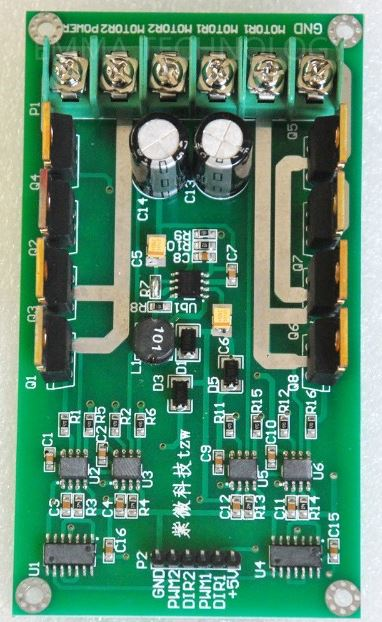
\includegraphics[angle=270,width=15cm]{driver1.JPG}
	\caption{Driver moteur}
	\label{fig:driver1}
\end{figure}

La partie commande (à gauche de la figure~\ref{fig:driver1}) possède 6 pins:

\begin{description}
	\item[GND \& +5V] Alimentation venant de la batterie;
	\item[PWM1 \& PWM2] Deux pins qui recoivent un signal MLI de deux autres pins de l'Arduino;
	\item[DIR1 \& DIR2] Spécifient le sens de rotation des moteurs. Elles peuvent être connectées à deux pins digitales de l’Arduino. Si elles reçoivent 0V, le moteur tourne dans un sens et pour 5V, le moteur tourne dans l’autre sens.
\end{description}

\paragraph{}
La partie puissance (à droite de la figure~\ref{fig:driver1}) possède également 6 bornes:

\begin{description}
	\item[GND \& POWER] Alimentation 24V venant de la carte d'alimentation;
	\item[2x MOTOR1] Connexion du premier moteur;
	\item[2x MOTOR2] Connexion du second moteur.
\end{description}

\paragraph{}
Sur chaque moteur, il est inscrit un "+" et un "-", on peut donc prendre une référence de polarité pour que les moteurs tournent dans le même sens. Par exemple, la borne "+" de chaque moteur connecté sur le bornier gauche de MOTOR1 et MOTOR2.

\subsubsection{Spécifications}\label{spec}
%~~~~~~~~~~~~~~~~~~~~~~~~~~~~~~~~~~~~~~~~~~~~~~~~~~~~~~~~~~~~
\begin{itemize}
	\item Alimentation de la partie puissance : 3-36V;
	\item Alimentation de la partie commande : 5V;
	\item Courant nominal : 10A;
	\item Courant de pointe : 30A;
	\item Commande : PWM (0-5V);
	\item Dimensions: longueur 108mm, largeur 58mm.
\end{itemize}

\paragraph{}
Nos moteurs sont alimenté en $24V$, leurs courants nominaux sont de $1.08A$, mais au démarrage, le pic de courant est de l'ordre de $11A$, soit $22A$ pour les deux moteurs ensemble.

\textbf{La carte driver répond à ces exigences}.

\subsection{Tests de fonctionnement}
%~~~~~~~~~~~~~~~~~~~~~~~~~~~~~~~~~~~~~~~~~~~~~~~~~~~~~~~~~~~~
Deux problèmes furent rencontrés et résolus. Le premier, le moteur changeait brusquement sa vitesse de rotation pendant une fraction de seconde lorsque le rapport cyclique changeait. Après de nouveaux tests au laboratoire d'électromécanique, il s'est avéré que le générateur de fonction fournissait une tension continue entre chaque transition de rapport cyclique. Ce qui avait pour effet de rendre les transistors de puissance passant à fond d'échelle pendant cette transition.
\noindent La solution apportée fût d'utiliser un autre générateur de MLI.

\paragraph{}
Le second problème est apparu lors du test complet entre Arduino - carte driver - moteur DC. Le moteur émettait un bruit, de plus, il tournait à basse vitesse alors que la consigne était de le faire tourner à sa vitesse maximum. Le diagnostic fût quasi immédiat, la fréquence du signal MLI était insuffisant. En effet, on n'a pu mesurer la fréquence du signal de comande à l'oscilloscope et elle était de l'ordre de 490Hz (fréquence par défaut provenant de l'arduino).

\paragraph{}
En modifiant certains registres internes de l'arduino, on est parvenu à modifier la fréquence de la MLI à 20kHz (fréquence qu'on peut changer à notre guise désormais). Finalement, le tout fonctionne correctement avec l'arduino qui fournit une MLI à 20kHz.